\documentclass[11pt,a4paper]{article}
\usepackage[margin=0.9in]{geometry}
\usepackage{graphicx}
\usepackage{amsmath,amssymb}
\usepackage[hidelinks]{hyperref}
\usepackage{xcolor}
\usepackage{booktabs,array}
\usepackage{caption}
\captionsetup[table]{font=small,labelfont=bf,skip=6pt}

\renewcommand{\topfraction}{0.9}
\renewcommand{\bottomfraction}{0.8}
\renewcommand{\textfraction}{0.08}
\renewcommand{\floatpagefraction}{0.75}
\setcounter{topnumber}{4}
\setcounter{totalnumber}{6}

\newcommand{\todo}[2]{\par\smallskip\begingroup\color{red!65!black}\raggedright\noindent\textbf{TODO #1:} #2\par\endgroup\smallskip}

% Figures from the final benchmark run are read directly from the results folder.
\graphicspath{{./}{../results/benchmark_20261109T113037Z/plots/}}

\title{Memory-Efficient Transformer Attention on CPUs\\[0.4em]
\large CEG5206: Algorithms \& Performance Optimization for Computing\\Group 11}
\author{Xinzhe Chen \quad Yikai Cao \quad Ziyi Yang \quad Peter Ong\\
\small National University of Singapore}
\date{November 2026}

\begin{document}
\maketitle

\section{Introduction}
% Problem, motivation and project scope.
Self-attention~\cite{vaswani2017} requires $\Theta(N^2d)$ arithmetic.
A direct implementation also stores an $N\times N$ score matrix, which occupies
64\,MiB in FP32 at $N=4096$ and exceeds the test CPU's 16\,MiB last-level cache.

We evaluate one unmasked FP32 attention head. Starting from a materialized
baseline (A), we add blocking and SIMD (B), tiled online softmax
(C)~\cite{milakov2018,rabe2021,dao2022}, and parallel execution (D).
Figure~\ref{fig:transformer-scope} shows the evaluated kernel within a Transformer.
All variants share an interface, FP64 reference and benchmark harness.

\begin{figure}[!htbp]
\centering
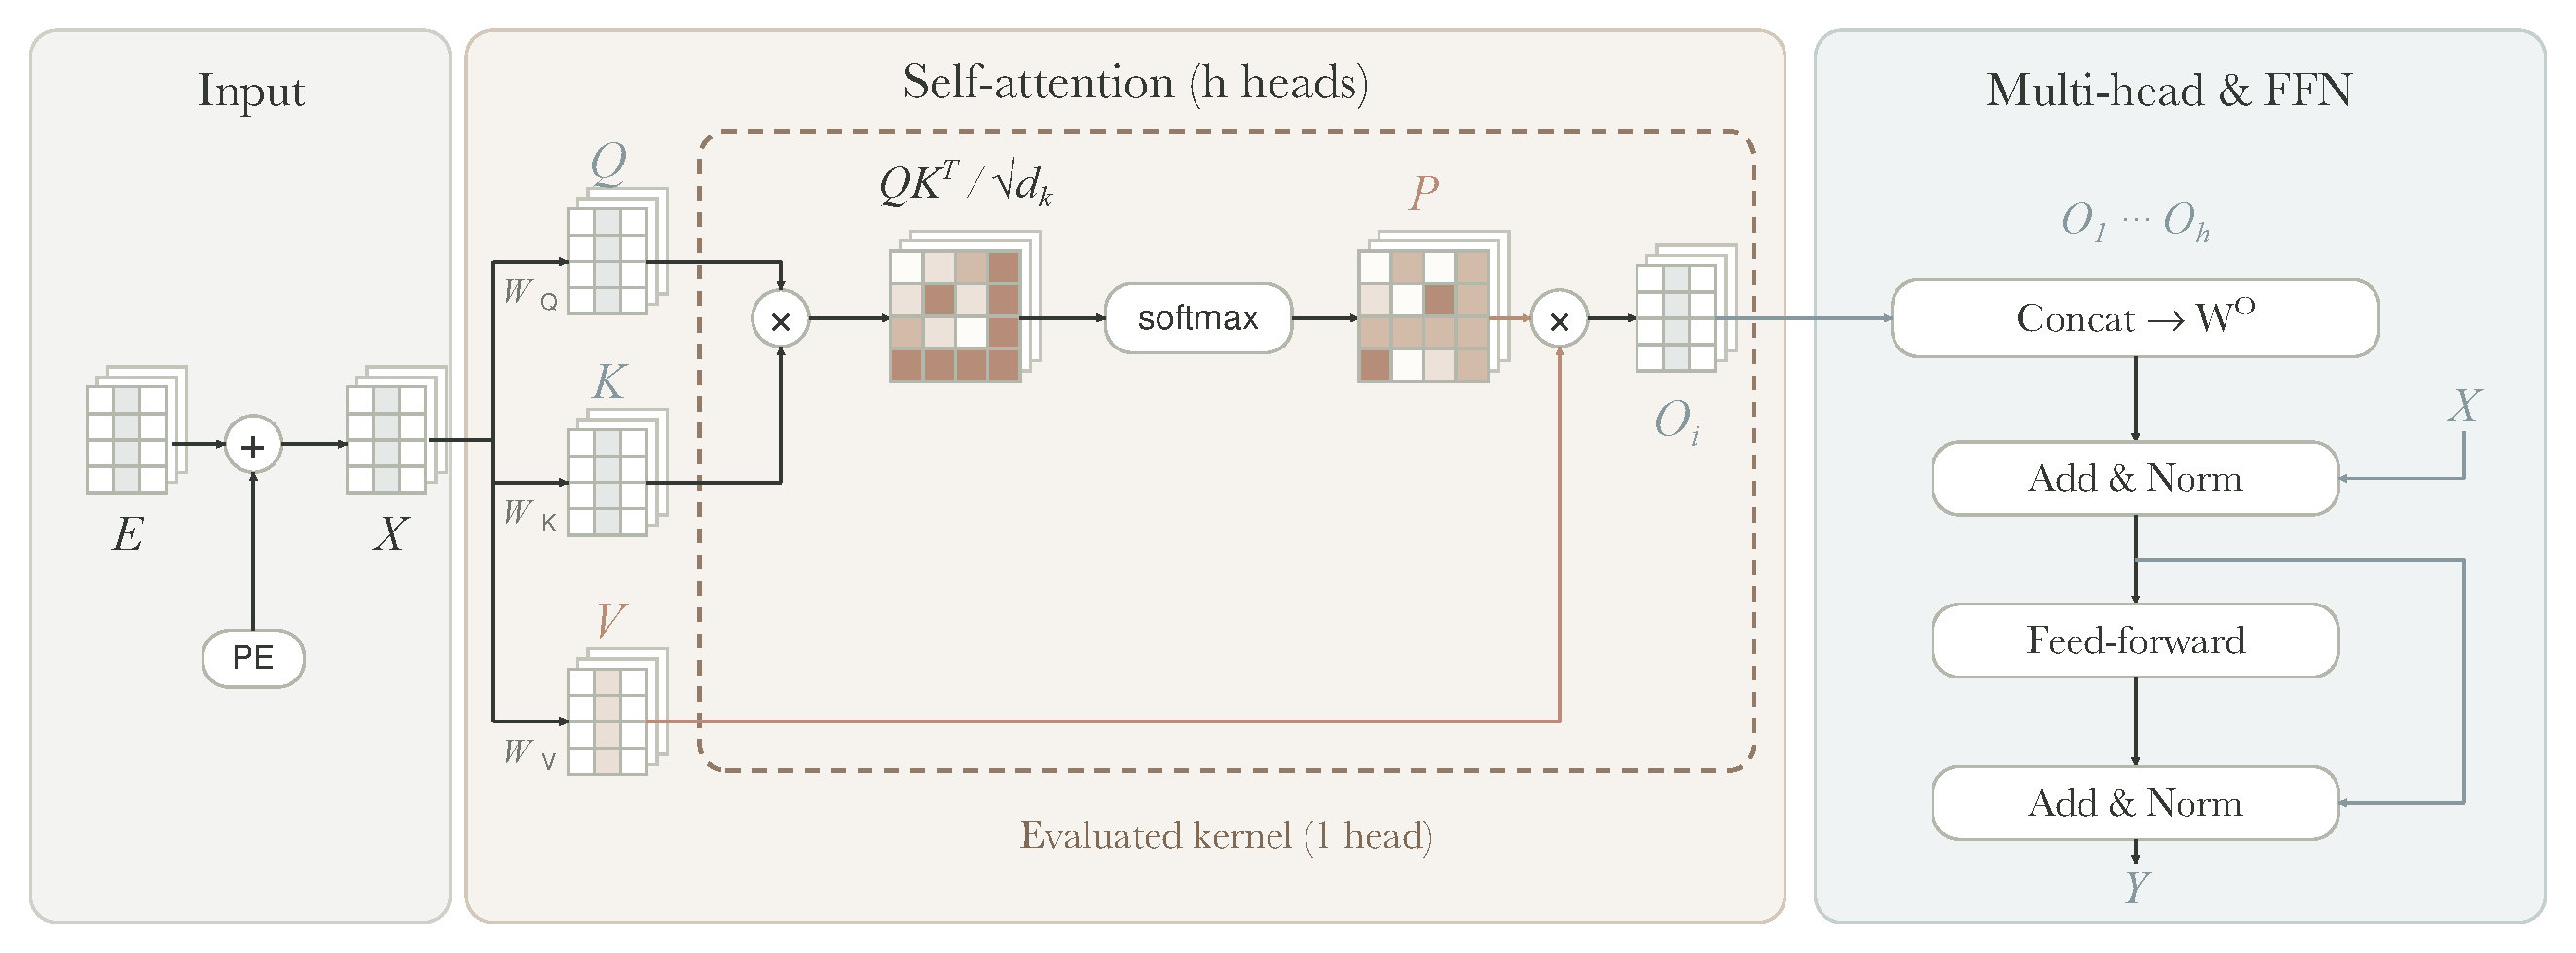
\includegraphics[width=0.94\linewidth]{transformer-connected.pdf}
\caption{Self-attention (left) and a post-norm Transformer block (right). Multi-head attention concatenates $h$ heads and applies $W_O$. Our experiments evaluate one unmasked head.}
\label{fig:transformer-scope}
\end{figure}

On an eight-core Intel Core i7-11700K, blocking and SIMD provide up to
$4.22\times$ single-thread speedup. Streaming reduces single-thread scratch
from 64\,MiB to 21--57\,KiB at $N=4096$. The best eight-thread variant reaches
$32.5\times$ speedup over the single-thread baseline.

\section{Implementation}
\subsection{Part A: Materialized Baseline}
The baseline computes single-head, unmasked attention for row-major matrices
$Q,K,V\in\mathbb{R}^{N\times d}$:
\[
O=\operatorname{softmax}\!\left(QK^{\mathsf T}/\sqrt{d}\right)V.
\]
It uses C++17 with FP32 inputs and accumulation, and runs with one thread.
Three stages compute the scaled dot products, apply row-wise softmax, and
multiply the probabilities by $V$. Softmax subtracts each row's maximum before
exponentiation for numerical stability. The score buffer is overwritten with
probabilities and reused across calls. Temporary storage is $4N^2$ bytes;
$Q$, $K$, $V$ and $O$ occupy a separate $16Nd$ bytes. The two matrix products
require approximately $4N^2d$ floating-point operations, excluding softmax
and scaling. Inputs are preserved, output is overwritten, and buffers are
allocated outside the kernel.

\subsection{Part B: Cache Blocking and Vectorization}
The blocked kernel retains the $4N^2$-byte score buffer. Query tiles contain
$B_r$ rows and key tiles contain $B_c$ rows. It computes scores with an
\texttt{omp simd reduction} across features, applies row-wise softmax in place,
then accumulates each $V$ tile across the query tile. The PV loop vectorizes
across contiguous features and preserves ascending key order.

Final tiles are clipped to the remaining rows, and feature loops handle SIMD
tails. All kernels use \texttt{-O3 -march=native}; single-thread SIMD builds use
\texttt{-fopenmp-simd}. A no-vec build disables SIMD hints and compiler
vectorization. A separate GCC~14.2 check at commit \texttt{d1f56ae} reports
32-byte vectors for both feature loops; timings use GCC~15.2.

The tuner validates nine pairs $B_r,B_c\in\{16,32,64\}$ at $(512,64)$ and
$(2048,64)$ on one thread. It minimizes geometric-mean median time relative
to $32\times32$ and selects $64\times32$ for both kernels. The full tuning step
takes about 45\,s. At $d=64$, one score tile's $Q$, $K$ and score data occupy
32\,KiB, compared with 48\,KiB L1D per core.

The reordered PV loop is the default. An optional packed-$K$ score loop
computes eight scores with independent accumulators, following panel
packing~\cite{goto2008}. Its benefit is evaluated separately.

\subsection{Part C: Streaming Attention}
The streaming kernel never stores more than one $B_r\times B_c$ tile of scores.
For each query tile it loops over key/value tiles and maintains, for every
query row $i$, a running maximum $m_i$, a running normalizer $\ell_i$ and an
unnormalized output vector $u_i\in\mathbb{R}^d$. For a new key tile with scores
$s_{ij}$, the online-softmax update~\cite{milakov2018} is
\[
m_i' = \max\!\Bigl(m_i,\max_j s_{ij}\Bigr),\quad
\alpha = e^{m_i-m_i'},\quad
\ell_i' = \alpha\,\ell_i + \sum_j e^{s_{ij}-m_i'},\quad
u_i' = \alpha\,u_i + \sum_j e^{s_{ij}-m_i'}\,v_j ,
\]
and after the last tile $O_i=u_i/\ell_i$. The result is exact softmax attention
up to floating-point rounding; no approximate exponential or fast-math flag is
used.

Two optimizations reduce the cost of this recurrence:
\begin{itemize}
\item \textbf{Packed $K$ tile.} Each key tile is transposed into a
  $B_c\times d$ panel in the worker's scratch. Eight adjacent scores are then
  computed with eight independent accumulators: one $Q$ element is multiplied
  by eight contiguous $K$ elements, which maps directly to vector FMA
  instructions. Remaining keys (fewer than eight) use an ordinary dot product.
  The panel is repacked for each query tile and the packing cost is included in
  the measured time.
\item \textbf{Conditional rescaling.} When a tile does not raise the running
  maximum, $\alpha$ is exactly 1, so the kernel skips both the exponential and
  the rescaling of $u_i$. The first tile starts from zeroed $\ell$ and $u$.
\end{itemize}

With $R=\min(B_r,N)$, $C=\min(B_c,N)$ and $W$ workers, the scratch buffer is
\[
4W\bigl(RC + Rd + 2R + Cd + 32[W>1]\bigr)\ \text{bytes},
\]
holding the score tile, $u$, $m$ and $\ell$, the packed $K$ panel, and a
128-byte gap between workers to avoid false sharing. For fixed tile sizes,
head dimension and thread capacity, scratch is bounded independently of $N$;
the exact allocation changes for small $N$ as $R$, $C$ and $W$ increase to their
caps. No memory is allocated inside the kernel. The caller reuses scratch
between calls, and the kernel keeps no additional persistent auxiliary arrays.

\subsection{Part D: Parallel Execution}
Both optimized kernels use an OpenMP static schedule over query tiles,
following the work partitioning in FlashAttention-2~\cite{dao2023}.
Each worker owns complete query rows and their state. Inputs are shared
read-only, blocked workers write disjoint score rows, and streaming gives
each worker padded scratch. Streaming uses
$W=\min(T,\lceil N/B_r\rceil)$ active workers for $T$ requested threads.

The per-row accumulation order is independent of thread count, enabling
bitwise repeatability for a fixed build and tile choice.
Timing uses \texttt{OMP\_PLACES=cores} and \texttt{OMP\_PROC\_BIND=close}.
The driver restores the CPU-affinity mask after NumPy import and records it
to prevent inherited affinity restrictions.

\section{Correctness Checks}
\subsection{Part A: Independent Reference and Tests}
An independent NumPy reference converts the exact FP32 inputs to FP64 and
computes the same attention operation. Every output element must satisfy
\[
|O_{ij}-O^{\mathrm{ref}}_{ij}|
\leq 10^{-4}+10^{-3}|O^{\mathrm{ref}}_{ij}|.
\]
The checks report maximum absolute and relative Frobenius errors and reject
NaN/Inf outputs. Cases include $N=1$, zeros, identical rows, signed random
inputs, non-divisible shapes $(127,33)$ and $(513,65)$, and concentrated
softmax distributions. The full grid covers
$N\in\{128,512,2048,4096\}$ and $d\in\{32,64,128\}$.
Additional checks cover invalid inputs and repeatability with reused buffers;
AddressSanitizer and UndefinedBehaviorSanitizer check memory safety and
undefined behaviour on the exercised paths.

\subsection{Parts B--D: Optimized and Threaded Kernels}
\label{sec:correct-bcd}
Both kernels use the same FP64 reference and tolerance. Tests cover partial
tiles, tiles of size 1 and larger than $N$, packed-loop tails, input preservation,
scratch reuse and online rescaling. The streaming API suite covers 201 serial
and 601 OpenMP configurations.

The benchmark gate passes 261 checks. Maximum absolute errors are
$8.3\times10^{-6}$ (baseline), $4.4\times10^{-6}$ (blocked) and
$1.1\times10^{-5}$ (streaming); the largest relative Frobenius error is
$1.51\times10^{-6}$. The edge/tile suite checks bitwise thread invariance at
2, 3, 8, 16 and 64 threads. The benchmark additionally checks eight-thread
invariance on all 12 core shapes. Clang~21.1.8 ThreadSanitizer with Archer
reports no issues on the tested paths.

R4 compares eight generated streaming variants to isolate score packing,
normalizer summation and maximum tracking. All 390 configurations pass.
On 36 random shape/seed cases, tile-local normalizer sums reduce relative
Frobenius error by 12.0--25.7\% versus sequential sums (20.6\% geometric mean).
This supports summation order as the main cause of the lower observed error
on those inputs. R4 is an untimed numerical diagnostic.

\section{Experimental Evaluation}
\subsection{Experimental Setup}
The test machine is an Intel Core i7-11700K with 8 cores, 16 hardware threads,
48\,KiB L1D and 512\,KiB L2 per core, and 16\,MiB shared L3. It runs Ubuntu
with GCC~15.2, performance governor and turbo disabled. Threads are pinned
to physical cores. Follow-up clock samples are near 3.6\,GHz, but do not
independently verify every short process.

The original ladder uses commit \texttt{bec3c57}, Linux~7.0.0-42 and a clean
working tree. Follow-ups R1--R6 use \texttt{eb8dc1d}; the six-round R3 rerun
uses \texttt{f460f4e}, with unchanged production kernel sources. Those sessions
run Linux~7.0.0-43 and are reported separately from the original ladder.

Each shape uses fixed-seed inputs from $[-1,1]$. After validation and five
warm-ups, variants rotate through three rounds of 15 timed samples each.
Short calls are batched to at least 10\,ms, capped at 1024 calls.
We report median per-call time and sample IQR. Timing reuses buffers and
includes packing, scratch initialization, softmax, normalization and OpenMP
fork/join. Allocation, validation and I/O are excluded. GFLOP/s uses $4N^2d$.

The median relative IQR across the 96 ladder rows is 0.4\%. Eight-thread
streaming at $(4096,32)$ has 37\% IQR because one round is slower.
An initial six-round rerun reproduces pooled medians within 0.3\%, but again
contains a slow all-core round. In R5's six monitored rounds, eight-thread
blocked medians range from 25.256 to 25.549\,ms and streaming from 20.399 to
20.567\,ms. The severe slowdown does not recur there; its cause remains open.
Pooled IQR measures sample spread rather than uncertainty across sessions.

\subsection{Reproduction}
\label{sec:repro}
The repository contains the source, tests, benchmark scripts, raw CSV files and
plotting scripts. With a C++17 compiler, GNU Make, Python and the pinned
\texttt{numpy}/\texttt{matplotlib} versions in \texttt{requirements.txt}, the
steps are, from the repository root:
\begin{verbatim}
python -m pip install -r requirements.txt
export PYTHON="$(which python)"
make test full sanitize
make OPENMP=1 test-streaming-api test-threads
make tsan
make benchmark
\end{verbatim}
\begingroup\raggedright
Machine preparation and the independent clock monitor are documented in
\texttt{docs/benchmarking.md} and \texttt{docs/report\_todos.md}.
The original tables and plots use
\path{results/benchmark_20261109T113037Z/}.
Initial follow-ups use \path{results/todo_20261110T000043Z/};
Table~\ref{tab:review-sources} lists later runs. Manifests retain source versions,
flags, validation and raw data. Independent clock summaries are under
\path{results/clock_audit_20261110/}. Follow-ups can be reproduced with
\begin{verbatim}
bash scripts/run_review_todos.sh --only R1 --threads 1,8
bash scripts/run_review_todos.sh --only R3 --threads 1,8 --rounds 6
\end{verbatim}

\endgroup

\begin{table}[!htbp]
\centering
\fontsize{9}{11}\selectfont
\setlength{\tabcolsep}{5pt}
\renewcommand{\arraystretch}{1.16}
\caption{New follow-up runs, each under \texttt{results/}. Run manifests name
the source version and settings; these data do not replace the original ladder.}
\label{tab:review-sources}
\begin{tabular}{@{}c l >{\raggedright\arraybackslash}p{0.30\linewidth}@{}}
\toprule
Task & \multicolumn{1}{c}{Directory} & \multicolumn{1}{c}{Evidence} \\
\midrule
R1 & \texttt{review\_20261110T023314094075Z} & Corrected counters and validation \\
R2 & \texttt{review\_20261110T054852698533Z} & Tile sweep and cache counters \\
R3 & \texttt{review\_20261110T052124567847Z} & Initial matched session \\
R3 & \texttt{review\_20261110T100054390740Z} & Six-round matched rerun \\
R4 & \texttt{review\_20261110T052530878469Z} & Numerical-factor experiment \\
R5 & \texttt{review\_20261110T052926748810Z} & Repeatability and telemetry \\
R6 & \texttt{review\_20261110T053132965490Z} & Controlled alignment and processes \\
\bottomrule
\end{tabular}
\end{table}

\subsection{Part A: Baseline Evaluation}
Table~\ref{tab:ladder} uses the serial baseline as the speedup reference.
It sustains 5.0--6.5\,GFLOP/s and runtime follows $N^2d$ over the tested shapes.
Score computation accounts for 73--76\% of its time
(Figure~\ref{fig:stages}). At $(4096,64)$, R1 records IPC 1.82,
18\% L1D misses and about 303\,MiB of DRAM traffic per call.

\begin{table}[!htbp]
\centering
\fontsize{9}{11}\selectfont
\setlength{\tabcolsep}{5pt}
\renewcommand{\arraystretch}{1.16}
\caption{Median time per call (ms) and speedup over the baseline. Tuned tiles
($64\times32$); threaded columns use 8 threads on 8 physical cores.}
\label{tab:ladder}
\begin{tabular}{@{}cc c cc cc cc cc@{}}
\toprule
 & & Baseline & \multicolumn{2}{c}{Blocked, 1T} & \multicolumn{2}{c}{Streaming, 1T}
 & \multicolumn{2}{c}{Blocked, 8T} & \multicolumn{2}{c}{Streaming, 8T} \\
\cmidrule(lr){4-5}\cmidrule(lr){6-7}\cmidrule(lr){8-9}\cmidrule(l){10-11}
$N$ & $d$ & ms & ms & $\times$ & ms & $\times$ & ms & $\times$ & ms & $\times$ \\
\midrule
128 & 32  & 0.328  & 0.180  & 1.82 & 0.147  & 2.23 & 0.091  & 3.59  & 0.075  & 4.39  \\
128 & 64  & 0.681  & 0.251  & 2.72 & 0.245  & 2.78 & 0.127  & 5.37  & 0.125  & 5.46  \\
128 & 128 & 1.609  & 0.382  & 4.22 & 0.452  & 3.56 & 0.187  & 8.60  & 0.230  & 7.01  \\
512 & 32  & 5.195  & 2.895  & 1.79 & 2.577  & 2.02 & 0.364  & 14.28 & 0.325  & 15.98 \\
512 & 64  & 11.388 & 4.270  & 2.67 & 3.828  & 2.97 & 0.538  & 21.18 & 0.502  & 22.71 \\
512 & 128 & 26.362 & 6.711  & 3.93 & 6.434  & 4.10 & 0.839  & 31.43 & 0.902  & 29.21 \\
2048 & 32  & 87.33  & 50.07  & 1.74 & 36.73  & 2.38 & 6.301  & 13.86 & 5.124  & 17.04 \\
2048 & 64  & 183.87 & 68.05  & 2.70 & 60.70  & 3.03 & 8.572  & 21.45 & 7.956  & 23.11 \\
2048 & 128 & 428.17 & 104.65 & 4.09 & 102.34 & 4.18 & 13.19  & 32.47 & 14.32  & 29.90 \\
4096 & 32  & 351.20 & 199.65 & 1.76 & 146.67 & 2.39 & 25.46  & 13.79 & 20.41  & 17.21 \\
4096 & 64  & 744.14 & 273.03 & 2.73 & 242.59 & 3.07 & 34.50  & 21.57 & 31.76  & 23.43 \\
4096 & 128 & 1712.4 & 419.13 & 4.09 & 410.25 & 4.17 & 52.93  & 32.35 & 57.22  & 29.93 \\
\bottomrule
\end{tabular}
\end{table}

\begin{figure}[!htbp]
\centering
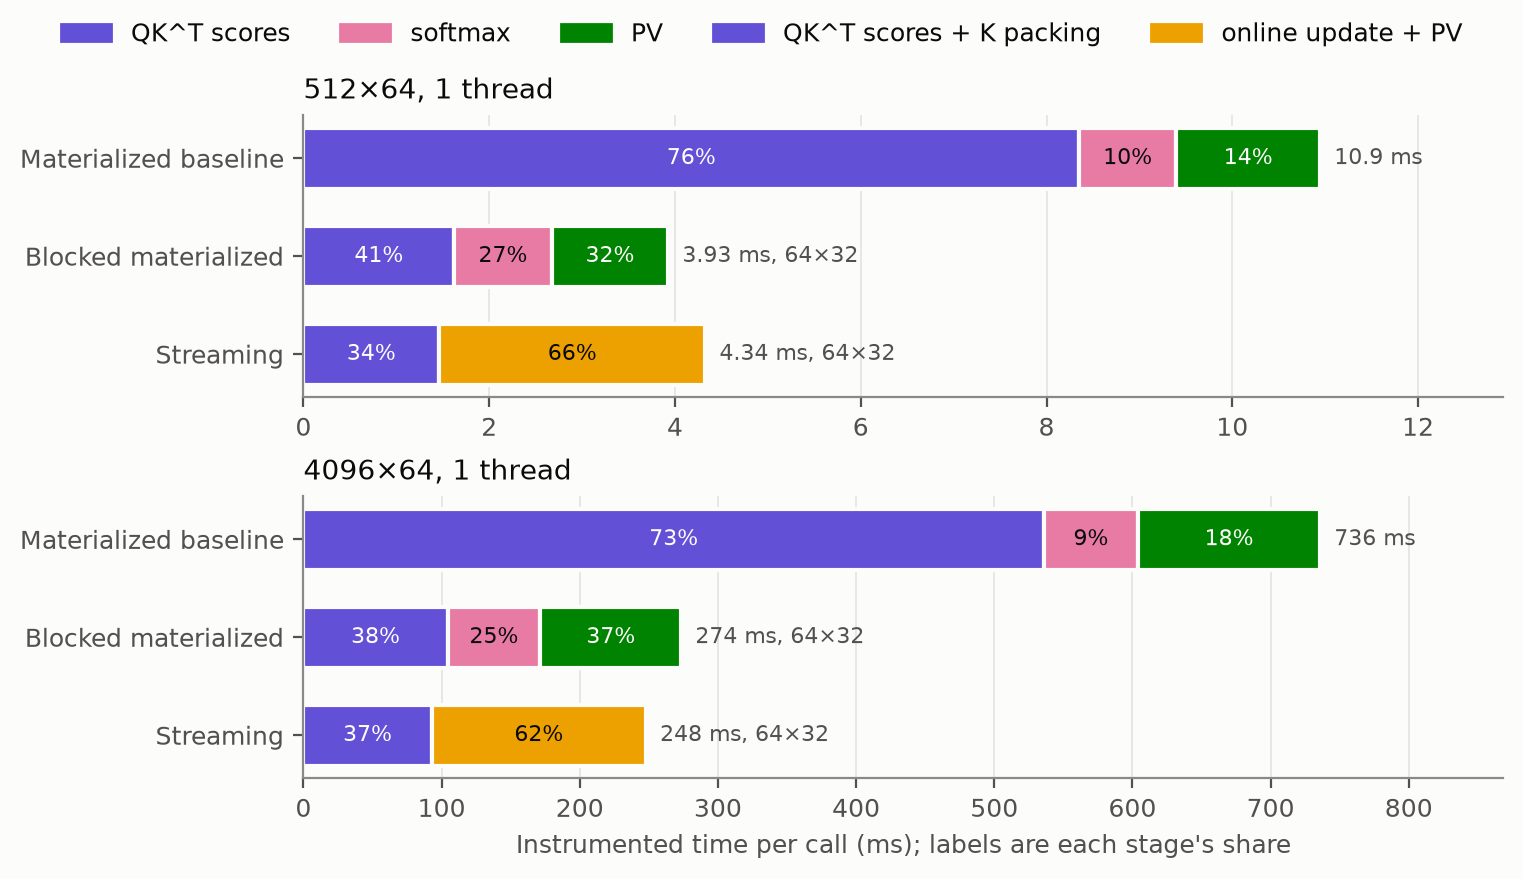
\includegraphics[width=0.72\linewidth]{stage_breakdown.png}
\caption{Instrumented per-stage time, one thread. Timers add overhead, so the
totals differ slightly from Table~\ref{tab:ladder}.}
\label{fig:stages}
\end{figure}

\subsection{Part B: Cache Blocking and Vectorization}
Blocking and SIMD improve single-thread time by $1.74$--$4.22\times$
(Figure~\ref{fig:speedup}), with larger gains at higher $d$.
At $(4096,64)$, the score stage is $5.1\times$ faster, leaving softmax at
about a quarter of blocked runtime (Figure~\ref{fig:stages}).

At $d=64$, disabling SIMD leaves blocked within 2\% of the baseline.
Enabling SIMD speeds up blocked by $4.7$--$5.0\times$, compared with
$1.7$--$1.8\times$ for baseline (Figure~\ref{fig:vec}).
The reordered PV loop reuses $V$ across queries. Packing $K$ is optional
because its benefit depends on head dimension, as tested by R3.

\begin{figure}[!htbp]
\centering
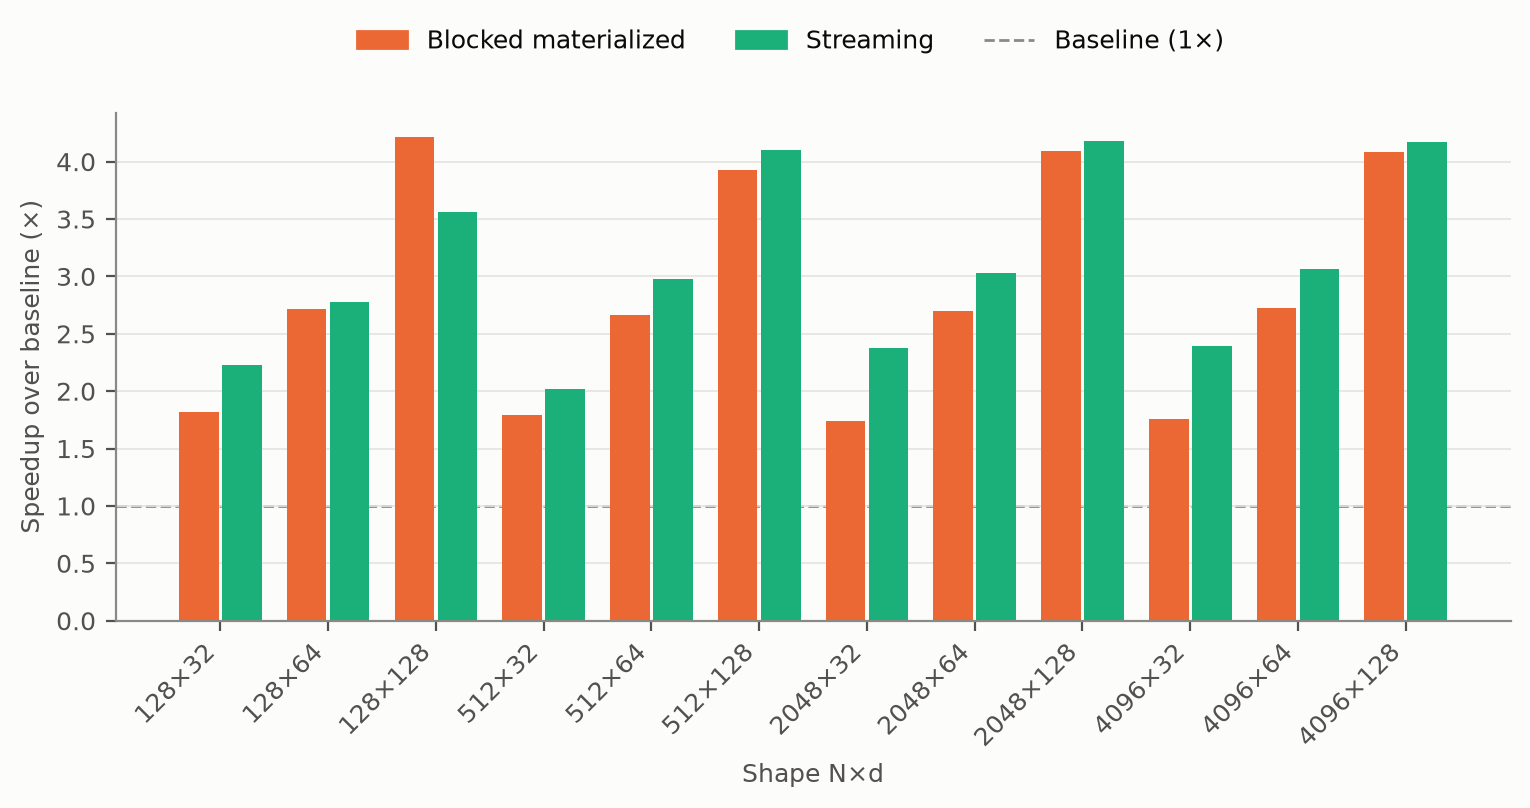
\includegraphics[width=0.72\linewidth]{speedup_1thread.png}
\caption{Single-thread speedup over the baseline for every shape.}
\label{fig:speedup}
\end{figure}

\begin{figure}[!htbp]
\centering
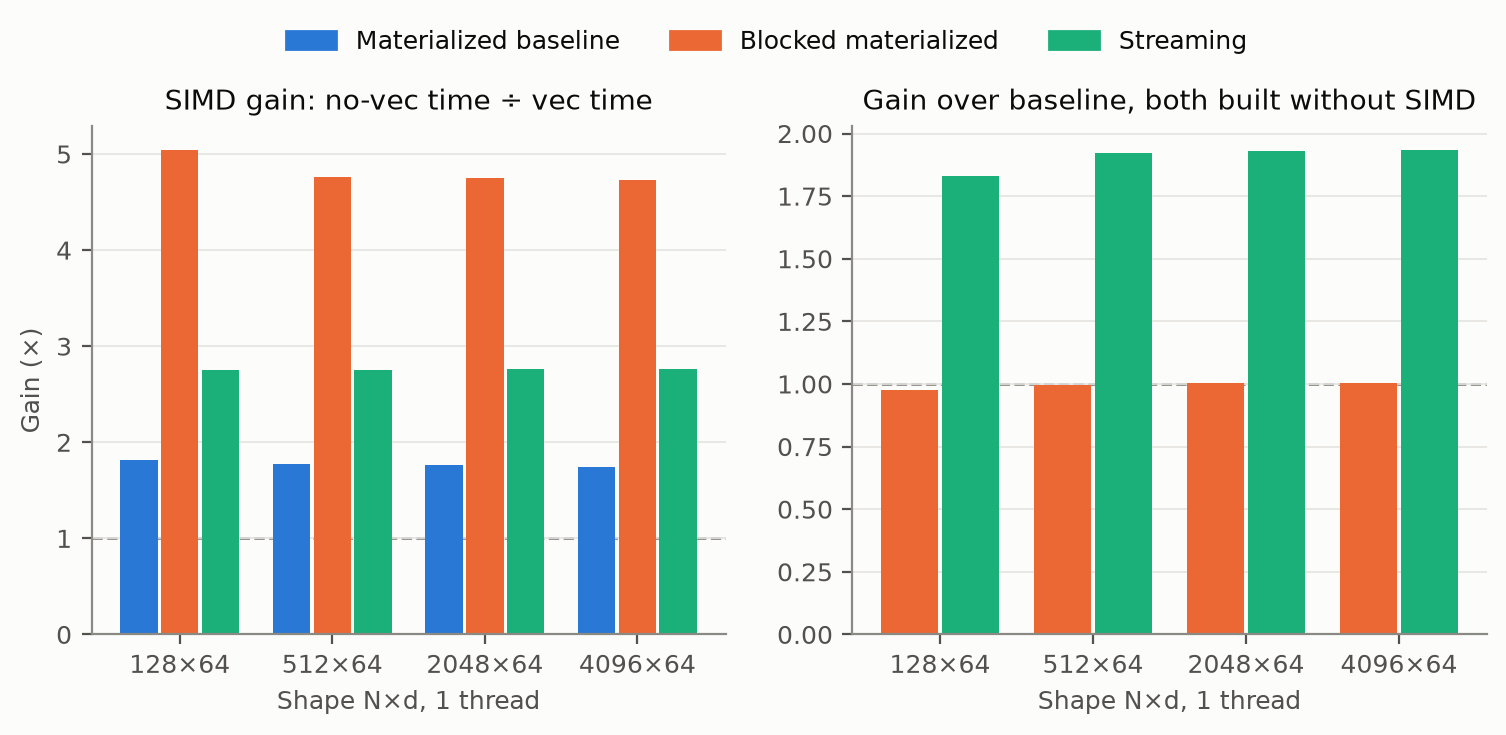
\includegraphics[width=0.72\linewidth]{vectorization.png}
\caption{Vectorization ablation, one thread. Left: speedup from enabling SIMD
in each kernel. Right: speedup over the baseline when all kernels are built
without SIMD.}
\label{fig:vec}
\end{figure}

\subsection{Part C: Streaming Attention}
\label{sec:eval-c}
Streaming uses 20.5, 32.5 and 56.5\,KiB of single-thread scratch for
$d=32,64,128$, constant over the tested sequence lengths
(Figure~\ref{fig:scratch}). Eight workers use at most 0.44\,MiB.
At $(4096,64)$, process peak RSS falls from 73.3 to 9.4\,MiB.
Corrected R1 counters measure about 0.8\,MiB of one-thread DRAM traffic
for streaming versus 146\,MiB for blocked. Small background-subtracted
traffic estimates are noisy.

Streaming is fastest on one thread in 11 of 12 original ladder shapes,
with $2.02$--$4.18\times$ speedup over baseline. The exception, $(128,128)$,
changes ranking across sessions. R6 tests six processes per variant,
five buffer offsets and two function alignments. Controlled 32-byte-aligned
buffers form a faster group, and blocked remains faster at matched offsets.
The original addresses were not logged, so alignment sensitivity does not
establish the cause of the earlier reversal.

\begin{figure}[!htbp]
\centering
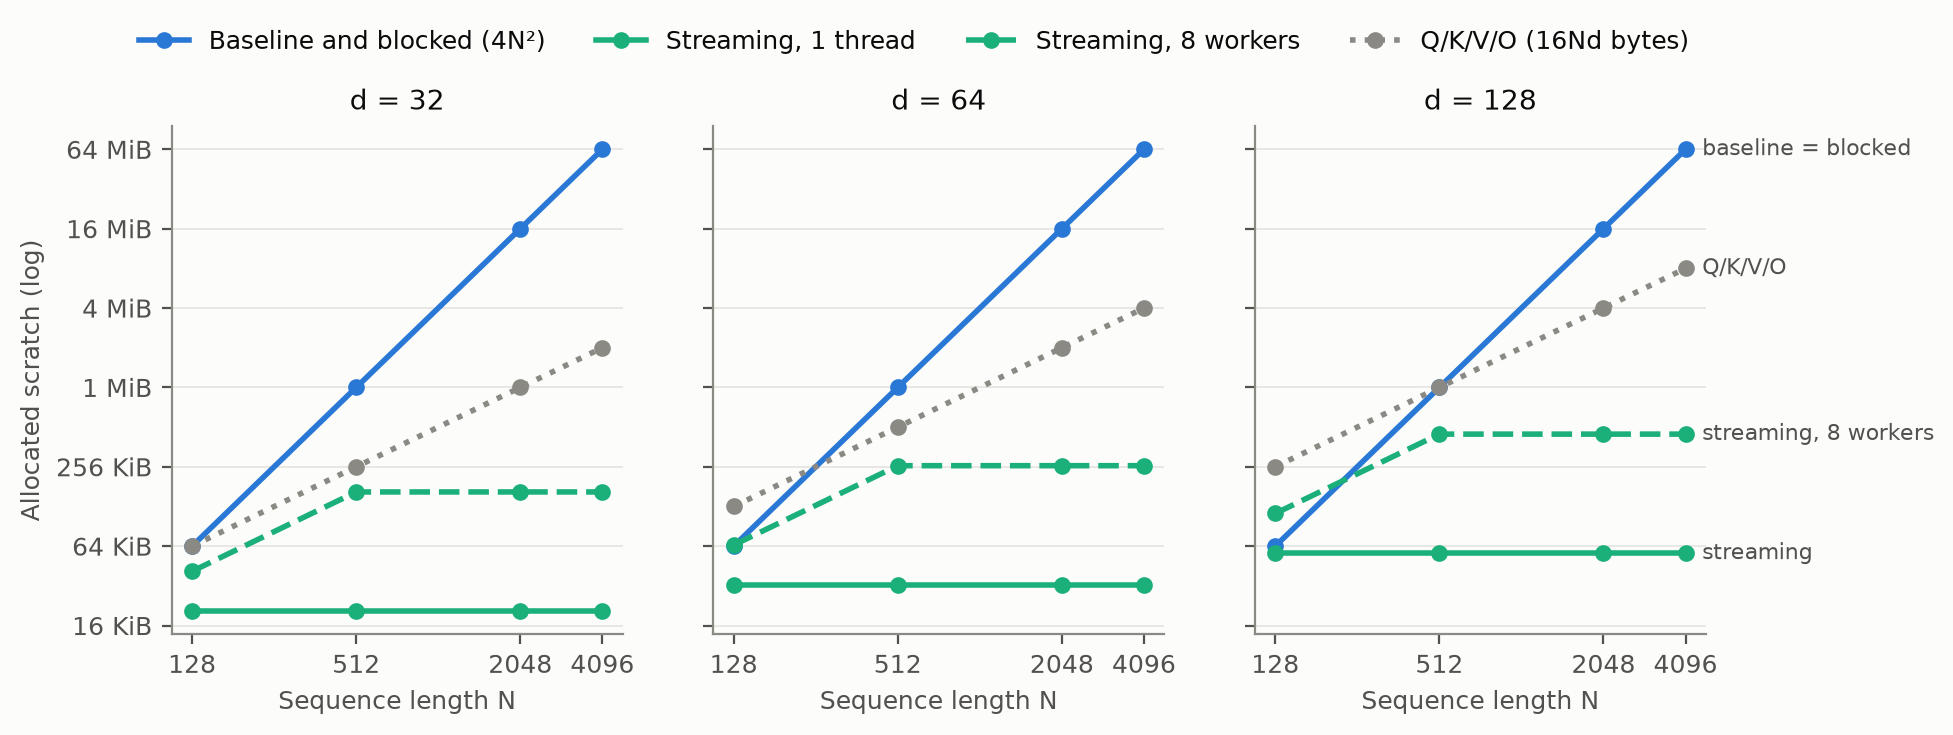
\includegraphics[width=0.85\linewidth]{scratch_vs_n.png}
\caption{Allocated kernel scratch against $N$ (log scale), with the $16Nd$
bytes of $Q$, $K$, $V$ and $O$ for reference.}
\label{fig:scratch}
\end{figure}

\paragraph{Matched score loops.}
R3 compares packed blocked with streaming using the same score-loop structure,
tiles, inputs and flags. The six-round rerun has 90 samples per variant and
passes all 24 validation configurations (Table~\ref{tab:matched}).
Streaming is $1.100$--$1.155\times$ faster on one thread.
On eight threads its advantage is about 5--7\% at $d\le64$, with near parity
at $d=128$. Some rounds remain disturbed, limiting claims about future sessions.
The residual gap includes normalization and update order as well as storage.

Instrumented profiles at $(4096,64)$ assign 37\% of streaming time to scores
and packing, and 62\% to online updates and PV (Figure~\ref{fig:stages}).
Without SIMD, streaming is still $1.8$--$1.9\times$ faster than the
unvectorized baseline at $d=64$; SIMD adds another $2.5$--$3.1\times$.

\begin{table}[!htbp]
\centering
\fontsize{9}{11}\selectfont
\setlength{\tabcolsep}{5pt}
\renewcommand{\arraystretch}{1.16}
\caption{Six-round R3 rerun, interleaved packed blocked versus streaming:
pooled median ms and blocked/streaming ratio, 90 samples per variant,
$64\times32$ tiles. A ratio above 1 means streaming is faster.
Sample spreads and residual round disturbances are discussed in the text.}
\label{tab:matched}
\begin{tabular}{@{}cc ccc ccc@{}}
\toprule
 & & \multicolumn{3}{c}{1 thread} & \multicolumn{3}{c}{8 threads} \\
\cmidrule(lr){3-5}\cmidrule(l){6-8}
$N$ & $d$ & blocked+pack & streaming & ratio & blocked+pack & streaming & ratio \\
\midrule
2048 & 32  & 42.107  & 36.595  & 1.151 & 5.377  & 5.116  & 1.051 \\
2048 & 64  & 66.711  & 60.541  & 1.102 & 8.378  & 7.984  & 1.049 \\
2048 & 128 & 112.767 & 102.508 & 1.100 & 14.182 & 14.324 & 0.990 \\
4096 & 32  & 168.701 & 146.111 & 1.155 & 21.889 & 20.400 & 1.073 \\
4096 & 64  & 269.944 & 242.367 & 1.114 & 33.803 & 31.763 & 1.064 \\
4096 & 128 & 451.599 & 409.142 & 1.104 & 57.132 & 57.206 & 0.999 \\
\bottomrule
\end{tabular}
\end{table}



\subsection{Part D: Parallel Scaling}
\label{sec:eval-d}
For $N\ge512$, moving from one to eight threads gives $7.84$--$8.00\times$
speedup for blocked and $7.13$--$7.92\times$ for streaming
(Figure~\ref{fig:scaling}, Table~\ref{tab:scaling}).
Blocked leads at $d=128$ on eight threads, while streaming leads at $d\le64$
in that range. At $N=128$, two query tiles limit useful parallelism to two workers.

R1 records little instruction-count growth from one to eight threads, but
streaming's total cycles rise by 4.7\% at $d=64$ and 12.8\% at $d=128$
(Table~\ref{tab:counters}). Its low DRAM traffic suggests that saturated DRAM
bandwidth does not explain the scaling loss. L2 miss counts include prefetches
and cannot isolate latency or coordination costs. Derived frequency ratios
also require the active worker count, especially at small $N$.

\begin{table}[!htbp]
\centering
\fontsize{9}{11}\selectfont
\setlength{\tabcolsep}{5pt}
\renewcommand{\arraystretch}{1.16}
\caption{Corrected R1 hardware counters per call at $N=4096$,
summed over all threads, pinned to physical cores. Counter groups use separate
passes. L2 misses include prefetch requests. Derived frequency ratios are not
used as independent clock measurements; small DRAM estimates are sensitive
to background subtraction.}
\label{tab:counters}
\begin{tabular}{@{}lcc ccccc@{}}
\toprule
Kernel & $d$ & $T$ & Gcycles & Ginstr. & IPC & L2 misses (M) & DRAM (MiB) \\
\midrule
Blocked & 64 & 1 & 0.991 & 2.979 & 3.01 & 11.93 & 146.4 \\
Blocked & 64 & 8 & 1.001 & 2.979 & 2.98 & 10.45 & 179.2 \\
Blocked & 128 & 1 & 1.505 & 4.456 & 2.96 & 13.25 & 151.6 \\
Blocked & 128 & 8 & 1.578 & 4.458 & 2.83 & 14.42 & 213.1 \\
\midrule
Streaming & 64 & 1 & 0.874 & 2.844 & 3.25 & 2.35 & 0.8 \\
Streaming & 64 & 8 & 0.915 & 2.846 & 3.11 & 2.38 & 1.0 \\
Streaming & 128 & 1 & 1.472 & 4.528 & 3.08 & 4.66 & 3.0 \\
Streaming & 128 & 8 & 1.660 & 4.533 & 2.73 & 4.78 & 0.4 \\
\bottomrule
\end{tabular}
\end{table}

\paragraph{Larger query tiles.}
R2 varies $B_r$ from 32 to 256 with $B_c=32$ (Table~\ref{tab:large-tiles}).
Increasing $B_r$ from 64 to 256 reduces eight-thread streaming time by about
2\%, despite much larger reductions in L2 misses. At $d=128$, it increases
serial time by about 8\% and eight-worker scratch from 0.44 to 1.39\,MiB.
These results support a trade-off rather than a universal tile optimum.
The original ladder retains $64\times32$ tiles.

\begin{table}[!htbp]
\centering
\fontsize{9}{11}\selectfont
\setlength{\tabcolsep}{5pt}
\renewcommand{\arraystretch}{1.16}
\caption{R2 streaming query-tile sweep at $N=4096,B_c=32$: pooled median
times (45 samples) and 8-thread L2 misses from separate counter passes.}
\label{tab:large-tiles}
\begin{tabular}{@{}cc ccc@{}}
\toprule
$d$ & $B_r$ & 1T ms & 8T ms & 8T L2 misses (M) \\
\midrule
64 & 32  & 248.143 & 32.343 & 4.61 \\
64 & 64  & 242.702 & 31.778 & 2.37 \\
64 & 128 & 239.649 & 31.366 & 1.21 \\
64 & 256 & 238.042 & 31.158 & 0.76 \\
\midrule
128 & 32  & 421.166 & 58.854 & 9.16 \\
128 & 64  & 409.674 & 57.206 & 4.77 \\
128 & 128 & 402.699 & 56.426 & 2.52 \\
128 & 256 & 442.237 & 56.126 & 2.70 \\
\bottomrule
\end{tabular}
\end{table}

R2's stall events also fail to isolate a shared-cache latency cause.
The remaining scaling loss may involve cache effects, dependency chains or
OpenMP coordination; their individual contributions remain unresolved.

\begin{table}[!htbp]
\centering
\fontsize{9}{11}\selectfont
\setlength{\tabcolsep}{5pt}
\renewcommand{\arraystretch}{1.16}
\caption{Thread scaling (data of Figure~\ref{fig:scaling}): median time per
call, interquartile range of the 45 samples, and speedup over the same kernel
on one thread. Threads pinned to physical cores, tuned $64\times32$ tiles.}
\label{tab:scaling}
\begin{tabular}{@{}ccc ccc ccc@{}}
\toprule
 & & & \multicolumn{3}{c}{Blocked} & \multicolumn{3}{c}{Streaming} \\
\cmidrule(lr){4-6}\cmidrule(l){7-9}
$N$ & $d$ & $T$ & ms & IQR (ms) & $\times$ & ms & IQR (ms) & $\times$ \\
\midrule
512 & 64 & 1 & 4.290 & 4.268--4.292 & 1.00 & 3.805 & 3.795--3.830 & 1.00 \\
512 & 64 & 2 & 2.130 & 2.128--2.141 & 2.01 & 1.919 & 1.916--1.921 & 1.98 \\
512 & 64 & 4 & 1.068 & 1.067--1.069 & 4.02 & 0.999 & 0.999--1.000 & 3.81 \\
512 & 64 & 8 & 0.539 & 0.538--0.540 & 7.97 & 0.501 & 0.501--0.502 & 7.59 \\
\midrule
4096 & 64 & 1 & 272.8 & 272.7--273.8 & 1.00 & 242.5 & 242.3--242.6 & 1.00 \\
4096 & 64 & 2 & 136.9 & 136.8--138.2 & 1.99 & 121.2 & 121.1--121.4 & 2.00 \\
4096 & 64 & 4 & 68.66 & 68.53--68.82 & 3.97 & 63.43 & 63.41--63.44 & 3.82 \\
4096 & 64 & 8 & 34.48 & 34.47--34.52 & 7.91 & 31.73 & 31.72--31.74 & 7.64 \\
\bottomrule
\end{tabular}
\end{table}

The best result in the original ladder is $32.5\times$ over baseline, reaching 163\,GFLOP/s, for blocked at $(2048,128)$ on eight threads.

\begin{figure}[!htbp]
\centering
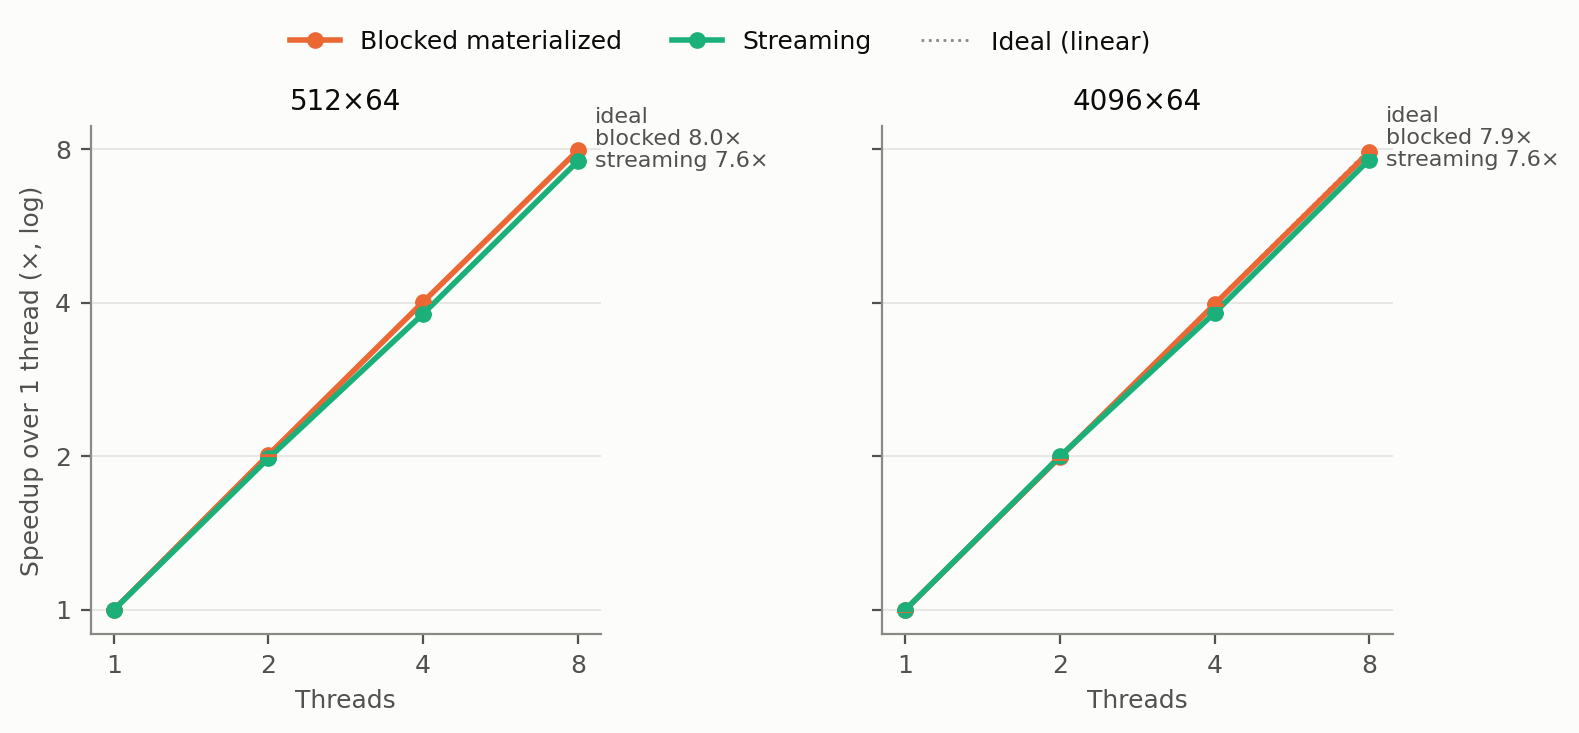
\includegraphics[width=0.72\linewidth]{thread_scaling.png}
\caption{Thread scaling relative to the same kernel on one thread, threads
pinned to physical cores. Error bars show the interquartile range of each
point; they are at most 1\% and mostly hidden by the markers.}
\label{fig:scaling}
\end{figure}

\subsection{Bottlenecks Against Compute and Memory Limits}
\label{sec:roofline}
A Roofline-style comparison~\cite{williams2009} uses a theoretical FP32 FMA
peak of 115\,GFLOP/s per core and 922\,GFLOP/s over eight cores at 3.6\,GHz.
The best kernel reaches 163\,GFLOP/s, about 18\% of that peak.
A 768\,MiB STREAM-style triad measures 25.1\,GB/s on one thread and
28.0\,GB/s on eight.

At $(4096,64)$, R1 gives model operational intensities of 13.5\,FLOP/B
for baseline, 28 for serial blocked, 23 for eight-thread blocked and over
4,000 for streaming. The eight-core ridge point is about 33\,FLOP/B, placing
blocked below a memory roof of roughly 640\,GFLOP/s. Its measured throughput
is 124\,GFLOP/s and bandwidth about 5.4\,GB/s.

Peak arithmetic and DRAM bandwidth are both underused. Stage profiles
identify substantial softmax and online-update work, but do not quantify a
unique bottleneck. Cheaper exponentials, updates and improved reuse remain
candidates requiring accuracy and performance validation. Materialized score
traffic scales with $N^2$, so increasing $N$ alone does not improve its
asymptotic operational intensity; increasing $d$ can.











\section{Conclusions and Limitations}
Blocking and SIMD accelerate the materialized kernel, while streaming removes
quadratic scratch and leads in 11 of 12 single-thread ladder cases.
Query-tile parallelism provides near-linear blocked scaling for $N\ge512$.
Follow-ups identify alignment sensitivity and numerical effects of normalizer
summation, and show that fewer cache misses alone give modest scaling gains.

The study covers one CPU, one unmasked FP32 head and $N\le4096$.
Small shapes are sensitive to process layout and available query tiles.
The tuned tiles and kernel rankings may change on other CPUs or workloads.
Matched score-loop timings still include normalization and execution-order
differences. Round disturbances and the remaining parallel-scaling gap are
unresolved. Masking, batching, multiple heads, projections and other precisions
require separate evaluation.

\section{Member Contributions}
The project applies established attention and online-softmax algorithms cited
above. Its technical work is the CPU implementation, loop and packing design,
thread ownership, validation, reproducible experiments and analysis.
\begin{center}
\fontsize{9}{11}\selectfont
\renewcommand{\arraystretch}{1.2}
\begin{tabular}{@{}l >{\raggedright\arraybackslash}p{0.70\linewidth}@{}}
\toprule
Member & Responsibility \\
\midrule
Chen Xinzhe & Baseline, FP64 reference and correctness tests \\
Yikai Cao & Cache blocking and vectorization \\
Ziyi Yang & Streaming attention and memory accounting \\
Peter Ong & Threading, benchmarking and profiling \\
\bottomrule
\end{tabular}
\end{center}

\section*{References}
% Add references and acknowledge adapted code or figures.
\begingroup
\renewcommand{\section}[2]{}
\begin{thebibliography}{9}
\bibitem{vaswani2017}
A.~Vaswani, N.~Shazeer, N.~Parmar, J.~Uszkoreit, L.~Jones, A.~N.~Gomez,
\L.~Kaiser and I.~Polosukhin.
\newblock Attention is all you need.
\newblock In \emph{Advances in Neural Information Processing Systems}, 2017.
\newblock \url{https://arxiv.org/abs/1706.03762}

\bibitem{milakov2018}
M.~Milakov and N.~Gimelshein.
\newblock Online normalizer calculation for softmax.
\newblock arXiv:1805.02867, 2018.

\bibitem{rabe2021}
M.~N.~Rabe and C.~Staats.
\newblock Self-attention does not need $O(n^2)$ memory.
\newblock arXiv:2112.05682, 2021.

\bibitem{dao2022}
T.~Dao, D.~Y.~Fu, S.~Ermon, A.~Rudra and C.~R\'e.
\newblock FlashAttention: Fast and memory-efficient exact attention with
IO-awareness.
\newblock In \emph{Advances in Neural Information Processing Systems}, 2022.

\bibitem{dao2023}
T.~Dao.
\newblock FlashAttention-2: Faster attention with better parallelism and work
partitioning.
\newblock arXiv:2307.08691, 2023.

\bibitem{goto2008}
K.~Goto and R.~A.~van~de~Geijn.
\newblock Anatomy of high-performance matrix multiplication.
\newblock \emph{ACM Transactions on Mathematical Software}, 34(3):12, 2008.
\newblock \href{https://doi.org/10.1145/1356052.1356053}{doi:10.1145/1356052.1356053}

\bibitem{williams2009}
S.~Williams, A.~Waterman and D.~Patterson.
\newblock Roofline: An insightful visual performance model for floating-point
programs and multicore architectures.
\newblock Technical Report UCB/EECS-2008-134, University of California,
Berkeley, 2008.
\end{thebibliography}
\endgroup

\noindent\textbf{Repository:} \url{https://github.com/ong-peter/ceg5206_group_project}\par
\todo{S3}{Add a clickable, accessible link to the 10--15-minute video covering
the approach, a demonstration, validation and main findings; verify that the instructor and TAs can access it.}
\noindent\textbf{Assessed source and report version:} \href{https://github.com/ong-peter/ceg5206_group_project/tree/ceg5206-report-2026-11-13}{\texttt{ceg5206-report-2026-11-13}}.\par
\noindent\textbf{Access and reproduction:} The repository and tagged report package are public. A clean checkout was used to verify the build, FP64-reference tests, streaming API and thread-invariance checks, and plot regeneration on Apple Silicon. These portability checks do not replace the reported Intel CPU measurements. Commands and validation logs are in \path{docs/submission_checks_2026-11-13.md}. Video access remains pending under S3.\par

\paragraph{AI assistance declaration.}
Generative AI assisted report formatting and editing.
\end{document}
